\newcommand{\maug}{\texttt{aug}\xspace}
\newcommand{\mcomp}{\texttt{comp}\xspace}

\definecolor{ccon}{HTML}{fee9d4}
\definecolor{cood}{HTML}{d8f0d3}
\definecolor{cid}{HTML}{dae8f5}

\newcommand{\TableAugSST}{
\begin{table*}
\small
\centering
\setlength{\tabcolsep}{4pt}
\begin{tabular}{@{}rrlllllllll@{}}
\toprule
    $n$ &     $m$ &    model & 
    \cellcolor{cid}SST-2 & 
    \cellcolor{cood}Senti140 & 
    \cellcolor{cood}SemEval & 
    \cellcolor{cood}Amzbook & 
    \cellcolor{cood}Yelp & 
    \cellcolor{cood}IMDB & 
    \cellcolor{ccon}IMDB-Cont. & 
    \cellcolor{ccon}IMDB-CDA \\
\midrule
 4,000 &  2,000 &     \mcomp &  $92.9\pm 0.2$ &  $88.9\pm 0.3$ &  $84.8\pm 0.5$ &  $85.1\pm 0.4$ &  $90.0\pm 0.3$ &  $90.8\pm 0.5$ &  $92.2\pm 0.6$ &  $86.5\pm 0.2$ \\
 4,000 &  2,000 &  \maug	 &  $92.7\pm 0.2$ &  $\mathbf{90.7\pm 0.4}$ &  $\mathbf{86.4\pm 0.1}$ &  $85.6\pm 0.8$ &  $90.1\pm 0.0$ &  $90.6\pm 0.3$ &  $\mathbf{94.0\pm 0.3}$ &  $\mathbf{89.7\pm 0.5}$ \\
 % imdb_contrast_test: 91.1 (9.4) / 92.8 (0.4)
 % imdb_contrast_test: 87.4 (0.0) / 89.6 (0.5)
 % imdb_iclr_test 93.0 (0.3) / 93.9 (0.4)
 % imdb_iclr_dev 92.0 (0.2) / 92.7 (0.2)
\bottomrule
\end{tabular}
\vspace{-5pt}
\caption{\sst model performances. 
\maug maintains the \colbox{cid}{in-domain} and \colbox{cood}{out-of-domain} accuracies on reviews (SST-2, Amzbook, Yelp, IMDb Movie Review~\cite{ni2019justifying, asghar2016yelp, maas2011learning}), but improves on Twitter data (Senti140 and SemEval 2017~\cite{go2009twitter, rosenthal2017semeval}), likely because their distributions are less similar to SST-2 than the reviews.
The model also improves on the \colbox{ccon}{contrast sets} (IMDb-Contrast and IMDb-CAD~\cite{gardner2020contrast, kaushik2019learning}).
%on \colbox{cid}{in domain}, \colbox{cood}{out of domain}, and \colbox{ccon}{contrast sets}. \maug performs better than \mcomp on twitter datasets (Senti140~\cite{go2009twitter}, SemEval 2017~\cite{rosenthal2017semeval}) and contrast sets IMDb-Contrast~\cite{gardner2020contrast} and IMDb-CAD~\cite{kaushik2019learning}, while maintaining the ones on reviews (SST-2, Amzbook~\cite{ni2019justifying}, Yelp~\cite{asghar2016yelp}, IMDb Movie Review~\cite{maas2011learning}).
}
\vspace{-5pt}
\label{table:aug_sst}
\end{table*}}

%%%%%%%%%%%%%%%%%%%%%%%%%%%%%%%%%%%%%%%%%%%%%%%
\newcommand{\TableAugNLI}{
\begin{table*}
\small
\centering
\setlength{\tabcolsep}{4pt}
\begin{tabular}{@{}rrlllllllll@{}}
\toprule
     $n$ &     $m$ &    model & \cellcolor{cid}SNLI & \cellcolor{cood}MNLI-m & \cellcolor{cood}MNLI-mm & \cellcolor{ccon}SNLI-CDA & \cellcolor{ccon}break & \cellcolor{ccon}DNC & \cellcolor{ccon}stress & \cellcolor{ccon}diagnostic \\
\midrule
 20,000 &  1,574 &     \mcomp 	&  $85.7\pm 0.4$&  $86.1\pm 0.2$&  $86.6\pm 0.2$&  $72.8\pm 0.3$&  $86.4\pm 1.5$&  $54.5\pm 0.6$&  $65.1\pm 0.6$&  $56.0\pm 0.8$\\
 20,000 &  1,574 &  \texttt{aug-r} &  $85.7\pm 0.4$ &  $86.1\pm 0.1$ &  $86.2\pm 0.1$ &  $73.4\pm 0.5$ &  $87.2\pm 0.6$ &  $54.7\pm 0.3$ &  $64.6\pm 0.6$ &  $56.9\pm 0.8$ \\
 20,000 &  1,574 &  \maug	&  $85.3\pm 0.3$&  $86.0\pm 0.1$&  $86.4\pm 0.0$&  $\mathbf{73.6\pm 0.2}$&  $\mathbf{89.1\pm 1.2}$&  $\mathbf{57.7\pm 0.3}$&  $65.1\pm 0.2$&  $\mathbf{57.5\pm 0.5}$\\
 %10000 &  1574 &     comp &  $85.3\pm 0.5$&  $85.2\pm 0.2$&  $85.4\pm 0.3$&  $72.4\pm 0.1$&  $86.1\pm 1.8$&  $54.2\pm 1.8$&  $64.0\pm 0.4$&  $56.0\pm 0.3$\\
 %10000 &  1574 &  aug\_gpt &  $85.3\pm 0.3$&  $85.0\pm 0.2$&  $85.1\pm 0.1$&  $73.4\pm 0.5$&  $90.5\pm 1.1$&  $56.5\pm 1.2$&  $64.6\pm 0.5$&  $57.0\pm 0.4$\\
\bottomrule
\end{tabular}
\vspace{-5pt}
\caption{\nli model performances. 
\maug performs better than \mcomp on DNC~\cite{kim2019probing}, which is the target of the augmentation. It also improves on other \colbox{ccon}{contrast/challenge sets}~\cite{naik2018stress, glockner-etal-2018-breaking, wang2018glue},  while maintaining the \colbox{cid}{in-domain} and \colbox{cood}{out-of-domain}~\cite{williams-etal-2018-broad} accuracies.}
\vspace{-5pt}
\label{table:aug_nli}
\end{table*}
}

%%%%%%%%%%%%%%%%%%%%%%%%%%%%%%%%%%%%%%%%%%%%%%%
\newcommand{\TableAugQQP}{
\begin{table}
\small
\centering
\setlength{\tabcolsep}{4pt}
\begin{tabular}{@{}p{0.4\textwidth} r@{}}
\toprule
TESTNAME &   $\Delta$ fail\%  \\
\midrule
 Order does not matter for symmetric relations &  -18.4\% \\
 Order does not matter for comparison &  -26.5\% \\
 Order does matter for asymmetric relations &  -14.5\% \\
%\midrule
% Is it \{ok, bad,..\} to \{smoke, do,..\} \{\emph{before $\not\eq$ after}\} &  -52.5\% \\
% %What was person's life \{\emph{before $\not\eq$ after}\} becoming X &  -46.6\% \\
% Do you have to X your dog \{\emph{before $\not\eq$ after}\} Y it &  -35.4\% \\
%\midrule
% Is person X $\not\eq$ Is person becoming X &  -8.5\% \\
% Is person X $\not\eq$ Did person use to be X &  -5.4\% \\
\midrule
 How can I become \{\emph{more X $\not\eq$ less X}\} &  -30.7\% \\
 How can I become \{\emph{more X $=$ less antonym(X)}\} &  28.0\% \\
 How can I become \{\emph{X $\not\eq$ not X}\} &  -10.4\% \\
 How can I become \{\emph{X $\not\eq$ not antonym(X)}\} &  -5.5\% \\
 %\midrule
 %traditional SRL: wrong active / passive swap &  2.2\% \\
 %traditional SRL: active / passive swap with people &  -6.4\% \\
 %traditional SRL: active / passive swap &  -15.2\% \\
%\midrule
 %Change first and last name in one of the questions &  -11.5\% \\
 %(q, paraphrase(q)) &  -5.3\% \\
\bottomrule
\end{tabular}
\vspace{-5pt}
\caption{
Sample \qqp CheckList tests~\cite{checklist:acl20}, with $\Delta$fail\% denoting the failure rate change from \mcomp to \maug. 
%However, the model gets significantly better on  \texttt{more X $\not\eq$ less X} by sacrificing \texttt{more X $=$ less antonym(X)}.
With $n=20,000$ and $m=1,911$, \maug reduced the failure rates on 11 tests (out of the 27 where \mcomp failed as defined in \S\ref{appendix:checklist}), while only increasing it for 2.
%Meanwhile, the models have similar accuracies on the test set ($84.5 \pm 0.6$ for \maug, and $84.7 \pm 1.0$ for \mcomp).
%Some sample tests are in Table~\ref{table:aug_qqp}.
The model improves consistently on most related cases, but possibly overfits on \texttt{more/less}.
}
\label{table:aug_qqp}
\vspace{-10pt}
\end{table}}


%%%%%%%%%%%%%%%%%%%%%%%%%%%%%%%%%%%%%%%%%%%%%%%
\section{\sysname for Training \& Evaluation}
\label{sec:app_label}
%\hao{suggestion: highlight the key results in 4.2, 4.3, and 4.4 upfront.}
Manually created counterfactuals are useful for evaluating and improving models~\cite{gardner2020contrast,kaushik2019learning}, but \emph{creating} variations is much more difficult than \emph{validating} them~\cite{ribeiro2018sear}.

Here, we ask crowdworkers to only label counterfactuals (\S\ref{subsec:label_efficiency}) that are automatically generated by \sysname (\S\ref{subsec:gen_counterfactual_for_labeling}).
We explore whether the labeled $\xp$ can support counterfactual evaluation (\S\ref{subsec:contrast_set}) and training (\S\ref{subsec:augmentation}), with experiments on three datasets (more in \S\ref{appendix:app_label_data}):
(1) \sst Analysis with Stanford Sentiment Treebank (\dsst)~\cite{socher2013recursive},
(2) Natural Language Inference (\nli) with \dnli~\cite{bowman-etal-2015-large}, and 
(3) Duplicate Question Detection (\dqqp)~\cite{wang2018glue}.
As \S\ref{subsec:label_takeaway} summarizes, the approach can serve the purposes at a much lower cost.

%\hao{the section below seems out of place}

\subsection{Selection for Labeling}
\label{subsec:gen_counterfactual_for_labeling}

%Not all counterfactuals have the same labeling utility, and we use the following two strategies to better compensate for the training space.

Starting with a set of $\xset$, our goal is to create a set of counterfactuals $\mathbf{L}$ for the crowdworker to label.
For each $x_i \in \xset$, we generate a large set of candidate counterfactuals $\hat{\xset}_i$, and sample three of $\xp \in \hat{\xset}_i$ to $\mathbf{L}$, such that crowdworkers label the same numbers of variations for each $x$.
To ensure we label the most effective counterfactuals, we \emph{generate} $\hat{\xset}$'s that target at models' known blind spots, and then \emph{select} the unique ones to form $\mathbf{L}$, as detailed below.

\textbf{Targeted counterfactuals.}
\citet{longpre2020effective} found that typical data augmentations are likely to bring redundant benefits as pre-training.
They suggested that the method should focus on where current models fail, which we follow in \S\ref{subsec:augmentation}.
We adjust \citet{chen2019slice}'s intuitive data slicing functions to find the $x$ with certain patterns of interest.
Then, we simply blank the corresponding patterns so \sysname can perform relevant changes.
For example, to highlight the impact of prepositions (\exinline{His surfboard is \swap{beneath}{lying on} him}), we first filter examples that have prepositions, and generate blanked prompts like \exinline{\ctrltag{[resemantic]} His surfboard is \texttt{[BLANK]} him.}


% (details in \S\ref{appendix:app_label_distance})
\textbf{Prioritize unique $\xp$.}
To cover more variations around local decision boundaries, we select unique counterfactuals through submodular optimization.
As mentioned in \S\ref{sec:general_purpose}, the selection is based on relationship $\relation{\xp}$.
In this case, it involves a set of components: \{\ the base $x$, tokens removed from $x$, added to $\xp$, the affected parsing tree structure, and the corresponding \tagstr.\ \}
We define a distance function on the relationships $D_L(\relation{\xp_i}, \relation{\xp_j})$, which is a weighted combination of the distances between each individual components.
Using $D_L[\boldsymbol{\cdot}]$, we greedily select $\xp$ whose $\relation{\xp}$ is the least similar to those already in $\mathbf{L}$.
For example, if \exinline{a \swap{man}{woman} walks} is already in $\mathbf{L}$, we would penalize \exinline{the \swap{man}{woman} is dancing} (same changed text) or \exinline{that dog is with the \swap{man}{girl}} (similar \ctrltag{lexical} change), but prioritize \exinline{\add{two} people talk.}



%The similarity computation is in \S\ref{appendix:perturb_similarity}. 
%\wts{Need to write this part.} 
%Formally, the distance between two counterfactuals is ($a_1$ is an abbreviation for $a(\xp_1, x)$):
%$$d(\xp_1, \xp_2) = \alpha\cdot\mathbb{1}(s_1 = s_2) + \beta\cdot\mathbb{1}(r_1 = r_2) + \gamma\cdot\mathbb{1}(a_1=a_2)$$
%With $\gamma = \beta > \alpha$ (empirically $2/5$, $2/5$, $1/5$).



\subsection{Labeling Procedure \& Efficiency}
\label{subsec:label_efficiency}

\textbf{Procedure.}
We crowd label the counterfactuals on Amazon Mechanical Turk. 
For each round, the annotator is given the original $x$ and its groundtruth as references\footnote{For \qqp and \nli, we only perturbed \emph{duplicate} and \emph{entailment} examples, as others are significantly harder to flip (called \emph{asymmetric counterfactuals}~\cite{garg2019counterfactual}).}, and is asked to label three counterfactuals by (1) the class label and (2) fluency (\emph{``likely written by a native English speaker''}). 
We carefully remove noisy workers using hidden \emph{gold rounds}, as well as filters on label distributions and completion time.
We also remove noisy labels through majority votes.
More details are in \S\ref{appendix:label_instruct}. 

\textbf{Fluency.}
Crowdworkers rated most counterfactuals to be fluent: $75\%$ for \dsst, $70\%$ for \dqqp, and $82\%$ for \dnli.
One of the authors also manually labeled 600 counterfactuals of 120 instances, and arrived at similar fluency:
The rate of unfiltered counterfactuals was $61\%$, which increased to $78\%$ after filtering, showing that the filtering is effective.

\textbf{Efficiency.}
Labeling three counterfactuals of a given example is reasonably easy, as (1) annotators are better at \emph{verifying} counterfactuals than manually \emph{generating} them~\cite{ribeiro2018sear}, and (2) annotators only need to focus on the reference example and the corresponding perturbed phrases, rather than re-parsing the full instance for each label they submit~\cite{Khashabi2020MoreBF}.
As such, the median time for labeling one round (three $\xp$) is 30 seconds.
Even in the most extreme (and very rare) case where we only keep 100 labeled $\xp$ that change the groundtruth after 500 rounds (\sst in \S\ref{subsec:contrast_set}), the average human annotation time per $\xp$ is 2.5 minutes, which is still 40\% more efficient than manual creation:
\citet{kaushik2019learning} reported that workers spent roughly 5 minutes to revise an IMDb review and 4 minutes a sentence (for \nli), even prior to additional filtering and validation.
%Similarly, \citet{gardner2020contrast} mentioned that three expert annotators spent 70 hours to create 588 counterfactual examples for IMDb review.

%Even for shorter image captions in NLVR2 visual reasoning dataset~\cite{suhr2018corpus}, annotations would take approximately 30 seconds for one textual perturbation.


%That said, manual creations are more flexible, and can take into account contexts beyond the prompt. 
%We discuss the opportunity for human-\sysname collaboration in \S\ref{sec:discuss}.




\begin{table}
\small
\centering
\setlength{\tabcolsep}{4pt}
\begin{tabular}{@{} c c c l c @{}}
\toprule
\textbf{Task} & \textbf{Dev.} & \textbf{Orig. set} & \textbf{Contrast set} & \textbf{Consistency} \\ 
\midrule
\sst & 94.3 & 93.8 & 84.9 (-8.9) & 76.1 \\
\nli & 86.5 & 91.6 & 72.3 (-19.3) & 56.4 \\
\qqp & 91.7 & 87.5 & 75.3 (-12.2) & 61.1\\
% \sst-distilbert & 91.1 & 93.2 & 84.0 (-9.2) & 75.0 \\
% \sst-bert & 92.4 & 90.9 & 85.8 (-9.2) & 76.1 \\
% \sst-roberta & 94.3 & 93.8 & 84.9 (-8.9) & 76.1 \\

% \nli-bert & 78.6 & 83.1 & 69.7 (-13.4) & 49.5 \\
% \nli-roberta & 86.5 & 91.6 & 72.3 (-19.3) & 56.4 \\
% \qqp-bert & 90.9 & 88.1 & 75.7 (-12.4) & 60.5 \\
% \qqp-distilbert & 89.7 & 88.1 & 72.4 & 57.3\\
% \qqp-roberta & 91.7 & 87.5 & 75.3 & 61.1\\
% the baseline
% \nli & 86.5 & 80.6 & 78.6 (-19.3) & 30.4 \\
% using a imdb model
% imdb_contrast_test 96.7 / 89.1 / 86.1
% imdb_iclr_test 96.7 / 91.0 / 87.9
% using a sst-2 model
% imdb_iclr_test 91.3 / 89.5 / 81.4
% imdb_iclr_test 89.5 / 87.3 / 77.3
\bottomrule
\end{tabular}
\vspace{-5pt}
\caption{Counterfactuals as contrasts sets, revealing model insufficiency. The table contains accuracies on the development set, the original $x$ (\emph{Orig. set}), the contrast sets, and the consistency between them.}
\vspace{-15pt}
\label{table:contrast_set_result}
\end{table}
%\end{comment}

\subsection{Experiment: Evaluation}
\label{subsec:contrast_set}

%%%%%%%%%%%%%%%%%%%%%
\TableAugSST
\TableAugNLI
%%%%%%%%%%%%%%%%%%%%%
Do \sysname counterfactuals serve as a useful test set for uncovering model errors?
\citet{gardner2020contrast} created \emph{contrast sets}, \ie minimally edited instances for inspecting model deficiencies, which we try to replicate.
Following the definition, we filter the counterfactuals to only keep those whose groundtruth label is different from $x$'s, resulting in contrast sets with sizes 100--300.
%: 106 $\xp$ on 88 $x$ for \sst, 276 $\xp$ on 202 $x$ for \nli, 243 $\xp$ on 185 $x$ for \qqp.
%We changed the \nli labels for 60\% of the time, whereas \sst was harder (only flipping 36.9\%).

%\paragraph{Models \& results.}
We test finetuned BERT~\cite{devlin-etal-2019-bert}, RoBERTa~\cite{liu2019roberta}, and DistilBERT~\cite{Sanh2019DistilBERTAD} models opensourced on Huggingface~\cite{Wolf2019HuggingFacesTS}, and report the best performing models on the validation set, which happen to be the RoBERTa model across tasks.\footnote{
\UrlFont{huggingface.co/\{roberta-large-mnli, textattack/roberta-base-SST-2,  ji-xin/roberta\_base-QQP-two\_stage\}}}
We report model accuracies on the full validation sets, the original examples for collecting counterfactuals, and the contrast sets.
We also report consistency, \ie cases where the model predicts both the originals and the counterfactuals correctly.
Table~\ref{table:contrast_set_result} shows that all state-of-the-art models perform significantly worse on our contrast sets, and the performance decreases for a similar amount as in \cite{gardner2020contrast}.
Results on other unreported models are consistent.
In other words, \sysname counterfactuals can reveal models' limited capabilities as the original contrast sets.


\subsection{Experiment: Training}

\label{subsec:augmentation}
%\paragraph{Collection.}
Do \sysname counterfactuals help yield better model generalization? 
We label counterfactuals for data augmentation.
Because counterfactuals that maintain the groundtruth can still improve model stability, we keep all the valid $\xp$ for one $x$, as long as at least one of them flips the groundtruth.

%\paragraph{Models.}
We finetune \texttt{roberta-base} models in HuggingFace.
For each augmented model (\maug), we include $m$ counterfactuals, as well as $n$ examples from the original dataset (the original $x$ of each $\xp$ will always be included).
Their baselines \mcomp replace the $m$ counterfactuals with another $m$ original examples.
Similar to \citet{Khashabi2020MoreBF}, this baseline helps evaluate whether labeling \emph{counterfactuals} is more effective than \emph{non-counterfactual} data.
The reported performances are averaged across multiple data samples and random seeds (More in \S\ref{appendix:data_collection}).
%Comparing with these models help highlight the effectiveness of perturbations with respect to adding the same amount of original data. 

\paragraph{Results.}
As shown in Table~\ref{table:aug_sst}--\ref{table:aug_qqp}, compared to adding the same amount of original data, \emph{the counterfactuals improve models' generalization} on out-of-domain datasets, challenge and contrast sets, as well as CheckList tests, while maintaining the in-domain accuracy.
%Critically, in \nli and \qqp, the improvement maintains even when the augmentation size is small (\eg when $m/n<10\%$).
Importantly, in both \nli and \qqp, \emph{just adding $m/n < 10\%$ data is sufficient to boost the performance.}

\TableAugQQP


\emph{However, targeted augmentation is necessary.}
While randomly generated counterfactuals are beneficial for \sst, similar to \citet{huang2020counterfactually}, they are not effective for either \nli or \qqp (numbers omitted for space.)
Instead, we apply the slicing strategy in \S\ref{subsec:gen_counterfactual_for_labeling} to prioritize counterfactuals related to known error cases, \eg prepositions in DNC~\cite{kim2019probing} for \nli, and entity orders in CheckList for \qqp.
The improved \maug in Table~\ref{table:aug_nli} and \ref{table:aug_qqp} indicates that such methods may help avoid repetitive augmentations.

\emph{The counterfactuals usually improve the model without hurting its counterpart.}
In \nli, DNC includes pairs of probing examples, one from the original MNLI and one manually and minimally perturbed.
%Because DNC includes both the probing counterfactuals and their paired original data, we can safely conclude that the model did not overfit to the augmented pattern.
The improvement on it shows that \maug did not overfit to the augmented pattern.
Similarly, the gain on CheckList tests are mostly consistent in \qqp (\eg all tests related to entity ordering were improved), except for the \texttt{more/less} contrast in Table~\ref{table:aug_qqp}.
Future work should further strategize the ranking to more equally cover competing patterns. 


\subsection{Takeaways}
\label{subsec:label_takeaway}

%Experiment results show that 
%, while saving at least 40\% of the creation time (\S\ref{subsec:label_efficiency}):

Our experiments show that \sysname supports both counterfactual evaluation and training.
More importantly, it achieves these at a noticeable lower cost, not only through shorter crowdlabeling time per instance, but also through targeted perturbation: data slicing and blanking help allocate the labeling efforts to best compensate the existing data, rather than wasting them on repetitive patterns.

\begin{comment}
\emph{The ratio of the counterfactuals matters. }
In both \nli and \qqp, just adding $m/n < 10\%$ data is sufficient to boost the performance.
In \sst, while the counterfactual remains effective on most datasets, it hurts the model performance on Amzbook when the counterfactual takes a large proportion (Figure~\ref{fig:sst_trend}, Yelp followed a similar but more mild trend).
We suspect that flipping out too much original data affects the data diversity, and in turn decreases the model performance.
Similarly, \citet{huang2020counterfactually} asserted that augmenting $n=1.7k$ NLI data with $m=6.6k$ counterfactuals did not improve model generalization accuracy over augmenting with non-counterfactual data.




\begin{figure}[t]
\centering
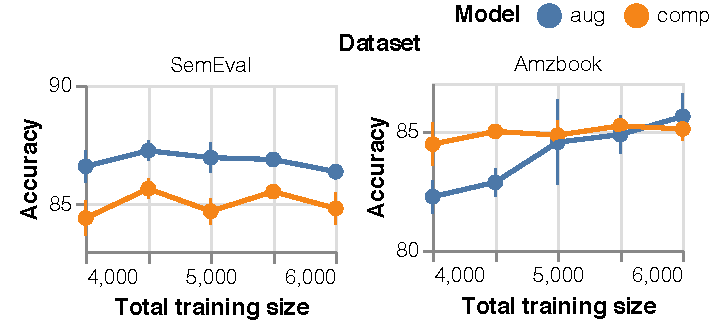
\includegraphics[width=1\columnwidth]{figures/sst_trend_2}
\vspace{-15pt}
\caption{The accuracy trend on \sst datasets, as the total training datasize $m+n$ varies. The blue line shows $m=2k$ \maug, and the orange one represents the corresponding \mcomp.
Though the counterfactuals remain useful on most datasets, too many counterfactuals may be harmful (\eg Amzbook when $m=n=2k$).
%\wts{Maybe cut/appendix?}
% (when $m+n=4k$, we have $m=n=2k$ on the orange line)
}
\vspace{-10pt}
\label{fig:sst_trend}
\end{figure}
\end{comment}

